\newpage
\section{Results}
\begin{figure}[H]
  \centering
    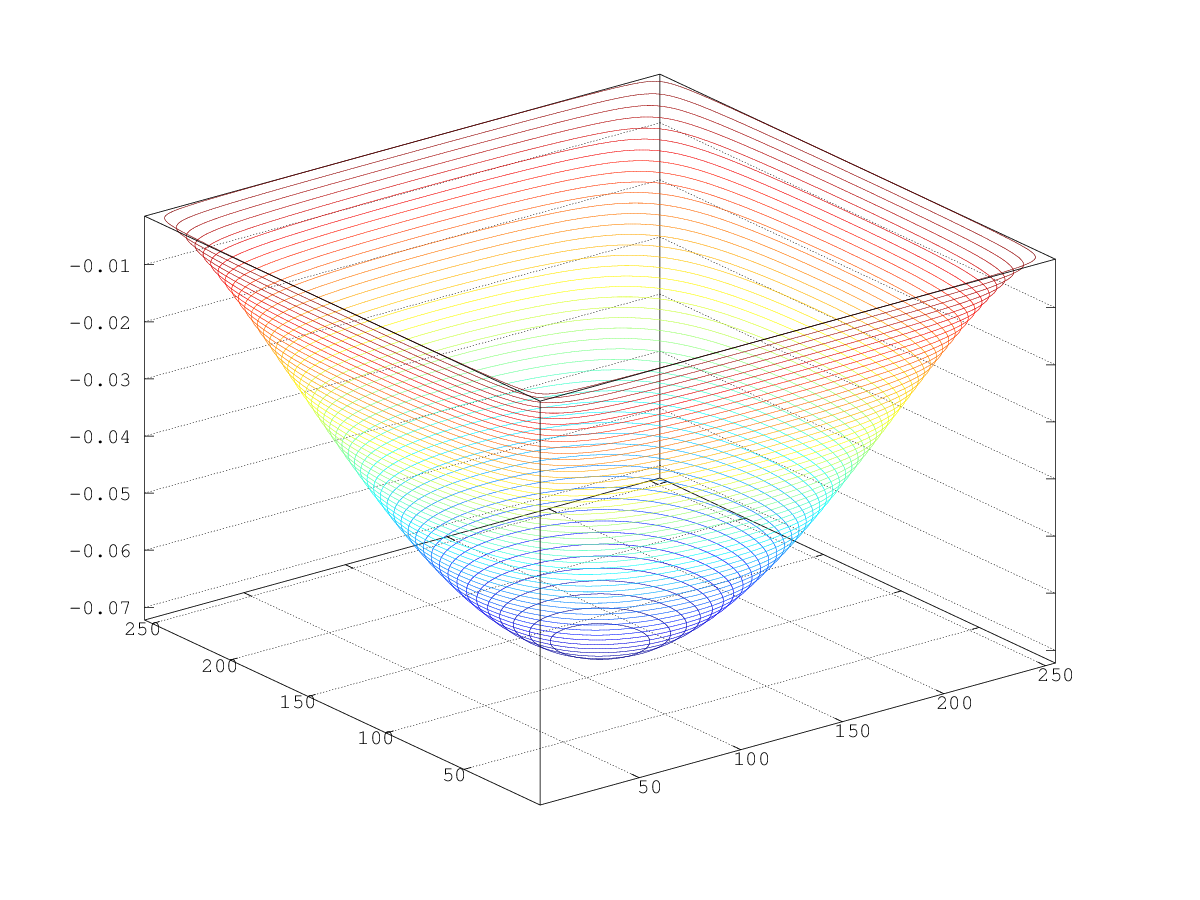
\includegraphics[width=0.7\textwidth]{datashit512flat_v2.png}
    \caption{$H^2$}
\end{figure}
\FloatBarrier
\begin{figure}[H]
  \centering
    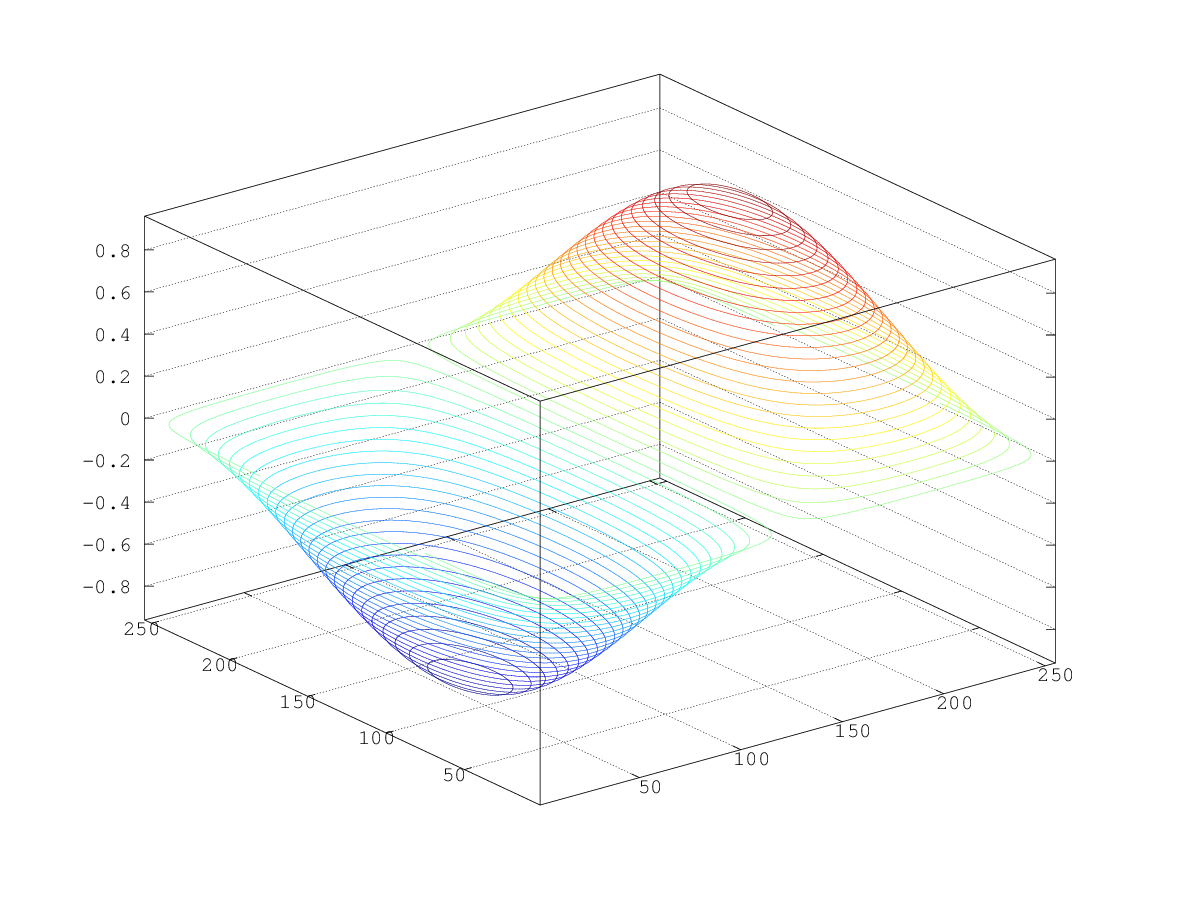
\includegraphics[width=0.7\textwidth]{datashit512sinpixsin2pix_v2.png}
    \caption{$(sin(\pi*x)\cdot sin(2\pi*y))\cdot 5\pi^2$}
\end{figure}
\FloatBarrier

\subsection{Speed}
We did some testing with various problem sizes to see how fast our program ran, then we
extrapolated the expected run time by using:
\begin{align}
k &= 
    \dfrac{n_{0}^2*\log{n_{0}}}{t}
\end{align}
\begin{align}    
t_{n} &= \dfrac
        {n^2\cdot\log{n}}
        {k} 
\end{align}

\begin{figure}[H]
  \centering
    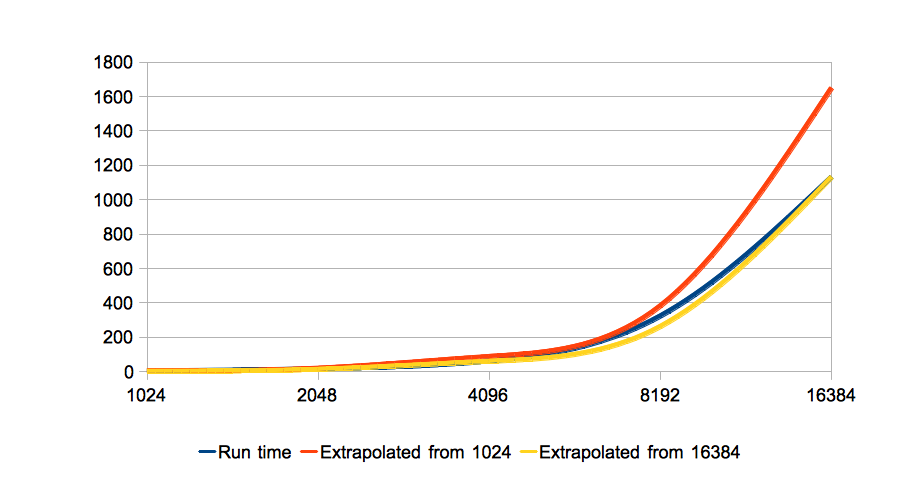
\includegraphics[width=0.8\textwidth]{speed_over_size_3.png}
    \caption{Run time for various problem sizes, compared to their extrapolation}
    \label{runsize}
\end{figure}

\begin{figure}[ht]
    \begin{tabular}{l | c | c | c | c}
        N & Run time & Extrapolated from 1024 & Extrapolated from 16384 & Speedup \\
        \hline
        1024 & 4,6 & 4,6 & 3,16\\
        2048 & 16,76 & 20,24 & 13,89 & 11,2522\\
        4096 & 62,8	 & 88,32 & 60,59 & 10,7935\\
        8192 & 323,67 & 382,72 & 262,55 & 4,1162\\
        16384 & 1130,97 & 1648,64 & 1130,97 \\
        \hline
    \end{tabular}
    \caption{Run time compared to extrapolated run time}
\end{figure}

To show a $n^2\cdot$log n extrapolation from the actual run time, as shown in figure \ref{runsize}, where we did an extrapolation from the run time of a problem set of size 1024 and up, and a similar extrapolation from the run time of a problem set of size 16 384. This shows that our runtime scales within the expected values, although the extrapolation looks closer when basing it on 16 384 than when basing it on 1024. This is partially because the smaller problem sets fit better into cache, but also because the actual run time dominates less than the constant-factors at these sizes.
\FloatBarrier
We also did a comparison with regards to how our program scales with the amount of processes it is run with,
as shown in figure \ref{numprocs4096}, our run time does indeed go down, with an odd increase in speed between 6 processes and 9 processes.
\begin{figure}[t]
  \centering
    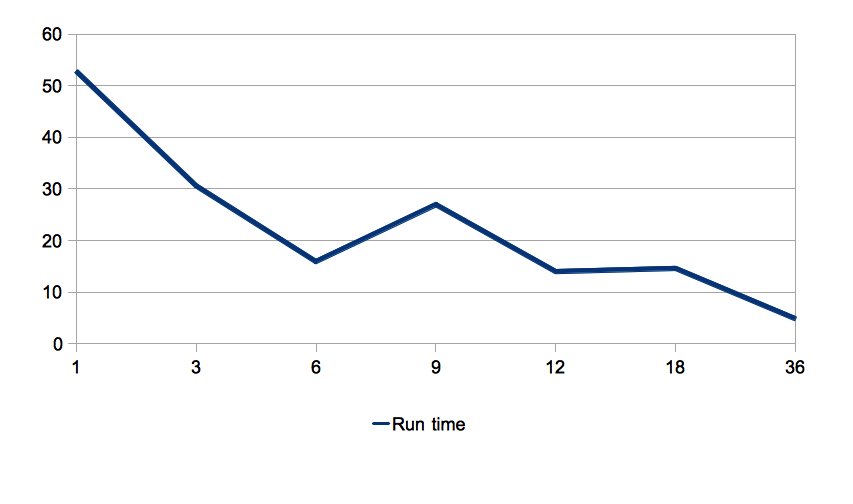
\includegraphics[width=0.8\textwidth]{RunTimePerProcess4096.png}
    \caption{Run time for problem size 4096 with varying process-amount}
    \label{numprocs4096}
\end{figure}

Similarly we did a comparison for problem sizes of 2048 (shown in Figure \ref{numprocs2048}, which showed a bit smoother a graph, mainly for the same reasons that the extrapolation from 1024 was weird, namely that we are quite a lot closer to the run times where the constant factors weigh more than the growth in problem size. This run also showed a similar local peak in the graph, around 18. The peaks shown in both these graphs might stem from variance in which node on Kongull runs our task, as, while
the Kongull-home page does state that it is a homogenous cluster, results and rumour seems to indicate that it is at least in part heterogenous, as some nodes seem to give a doubling in floating point operation-speed compared to other nodes. Rerunning the tests provided different results, which leads us to thinking that the rumours are true. Either way, the results shown here are all from the same batch-job, prioritizing consistency before averaging out such errors.

A similar run was also run for problem sizes of 8192 (Figure \ref{numprocs8192} ).

\begin{figure}[H]
  \centering
    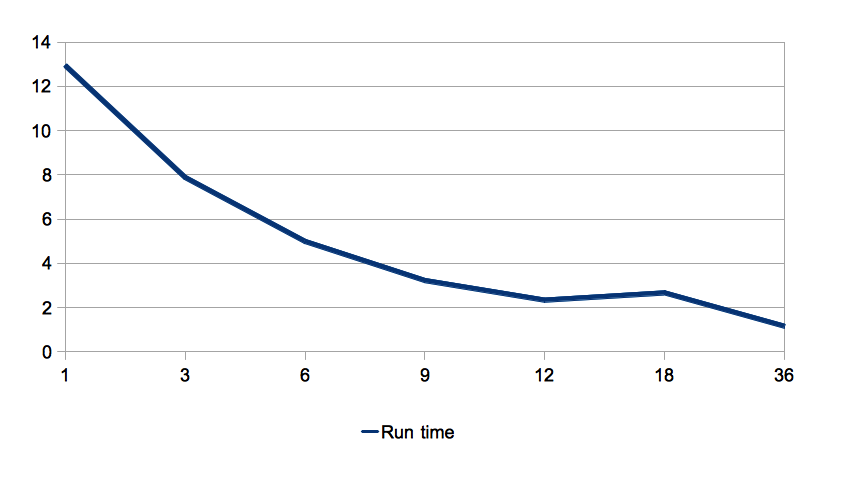
\includegraphics[width=0.8\textwidth]{RunTimePerProcess2048.png}
    \caption{Run time for problem size 2048 with varying process-amount}
    \label{numprocs2048}
\end{figure}

\begin{figure}[t]
  \centering
    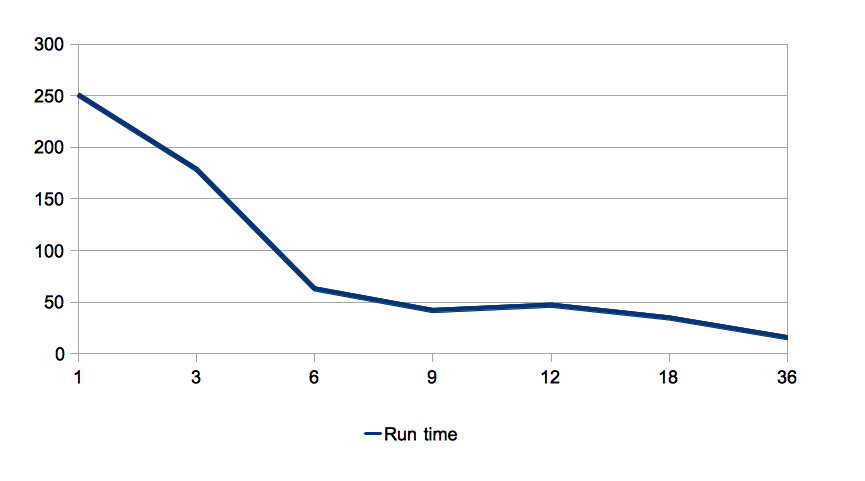
\includegraphics[width=0.8\textwidth]{RunTimePerProcess8192.png}
    \caption{Run time for problem size 2048 with varying process-amount}
    \label{numprocs8192}
\end{figure}

\begin{table}[ht]
    \begin{tabular}{l | c | c | r}
        NumProcs & Speed & SpeedUp & Parallell Efficiency \\
        \hline
        1 & 12,94 & 1 & 1 \\
        3 & 7,88 & 1,6421 & 0,547 \\
        6 & 4,99 & 2,5932 & 0,432 \\
        9 & 3,22 & 4,0186 & 0,44651 \\
        12 & 2,33 & 5,5536 & 0,46280 \\
        18 & 2,66 & 4,8647 & 0,27026 \\
        36 & 1,15 & 11,2522 & 0,31256 \\
        \hline
    \end{tabular}
    \caption{Speedup and parallell efficiency for problem size 2048}
\end{table}

\begin{table}[ht]
    \begin{tabular}{l | c | c | r}
        NumProcs & Speed & SpeedUp & Parallell Efficiency \\
        \hline
        1 & 52,78 & 1 & 1 \\
        3 & 30,59 & 1,7254 & 0,575 \\
        6 & 15,4 & 3,3195 & 0,55325 \\
        9 & 26,95 & 1,4584 & 0,21760 \\
        12 & 13,98 & 3,7754 & 0,31462 \\
        18 & 14,59 & 3,6175 & 0,20097 \\
        36 & 4,84 & 10,7935 & 0,24982 \\
        \hline
    \end{tabular}
    \caption{Speedup and parallell efficiency for problem size 4096}
\end{table}

\begin{table}[ht]
       \begin{tabular}{l | c | c | r}
        NumProcs & Speed & SpeedUp & Parallell Efficiency \\
        \hline
        1 & 250,8 & 1 & 1 \\
        3 & 178,74 & 1,4032 & 0,46772 \\
        6 & 62,89 & 3,9879 & 0,66465 \\
        9 & 41,92 & 5,9828 & 0,66476 \\
        12 & 47,12 & 5,3226 & 0,44355 \\
        18 & 34,74 & 7,2193 & 0,40107 \\
        36 & 15,58 & ? & ? \\
        \hline
    \end{tabular}
\caption{Speedup and parallell efficiency for problem size 8192}
\end{table}
\FloatBarrier